\subsection{Eksempel på basisproblemet} \label{kap:graf_basis}
Vi kan med udgangspunkt i afsnittet om grafteori opstille en graf for vores basisproblem. Grafen er en simpel, orienteret og vægtet graf. Vi opstiller et simplificeret eksempel på grafen for at demonstrere, hvordan et problem af vores type kan løses med grafteori. I eksemplet arbejder vi med følgende data:
\begin{itemize}
  \item $t \in \{1,2,3,4,5,6\}$
  \item $q_{0}=1$
  \item $q_{\min}=0$
  \item $q_{\max}=2$
  \item $i_{\max}=1$
  \item $u_{\max}=1$
  \item $p_{6}=(20,22,25,18,15,15)$
\end{itemize}

I vores eksempel tager vi kun udgangspunkt i seks måneder, og at man kun kan købe og sælge en gasenhed pr. måned. Derudover er lageret begrænset til mindst at have nul gasenheder og højst at have to gasenheder. Efter de seks måneder sælger vi det gas, der muligvis er tilbage på lageret til ejeren. Vi opstiller følgende graf med de givne vægte:

\input{fig/tikz/gaslager/forsimplet_graf}

Hvis vi skal maksimere resultatet for dette gaslager, ønsker vi at finde den længste vej fra $q_{0}$ til $q_{\slut}$, da vi skal have så stort overskud som muligt efter endt lejeperiode. For at løse problemet som et korteste vej-problem og ikke et længste vej-problem ganger vi med -1. Vi opstiller dermed den omvendte graf for problemet:

\begin{figure}[H]
\centering
	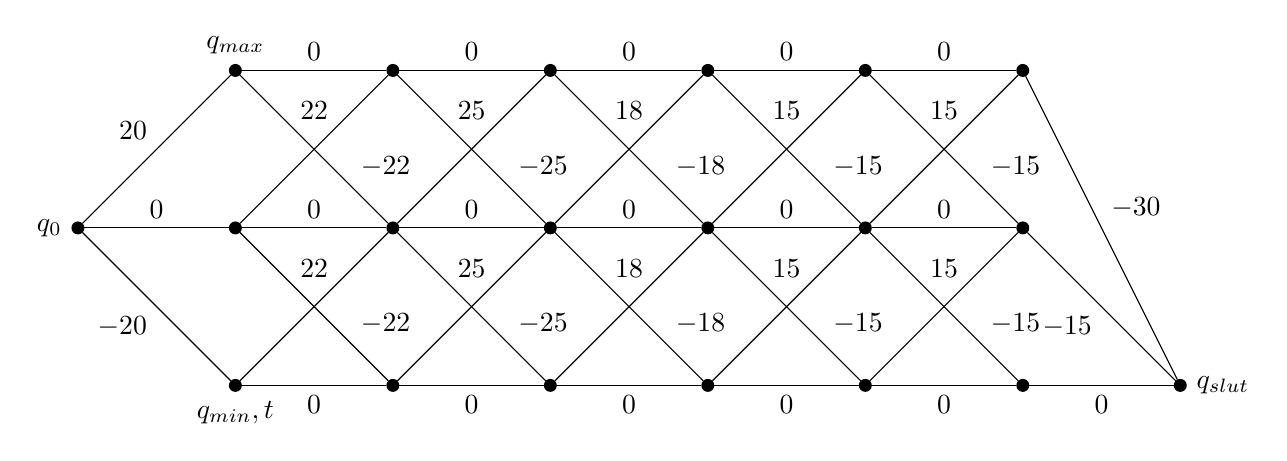
\begin{tikzpicture}

      \tikzset{enclosed/.style={draw, circle, inner sep=0pt, minimum size=.15cm, fill=black}}
%% Vertices
      	\node[enclosed, label={left: $q_{0}$}] (v1) at (0,2) {};
      	\node[enclosed, label={below: $q_{min},   t$}] (v2) at (2,0) {};
    		\node[enclosed, label={below: }] (v3) at (2,2) {};
  	    \node[enclosed, label={above: $q_{max}$}] (v4) at (2,4) {};
     	\node[enclosed, label={left: }] (v5) at (4,0) {};
     	\node[enclosed, label={left: }] (v6) at (4,2) {};
     	\node[enclosed, label={left: }] (v7) at (4,4) {};
     	\node[enclosed, label={right: }] (v8) at (6,0) {};
     	\node[enclosed, label={right: }] (v9) at (6,2) {};
     	\node[enclosed, label={right: }] (v10) at (6,4) {};
     	\node[enclosed, label={right: }] (v11) at (8,0) {};
     	\node[enclosed, label={below: }] (v12) at (8,2) {};
      	\node[enclosed, label={below: }] (v13) at (8,4) {};
  	    \node[enclosed, label={below: }] (v14) at (10,0) {};
  	    \node[enclosed, label={below: }] (v15) at (10,2) {};
     	\node[enclosed, label={below: }] (v16) at (10,4) {};
     	\node[enclosed, label={below: }] (v17) at (12,0) {};
     	 \node[enclosed, label={below:}] (v18) at (12,2) {};
     	\node[enclosed, label={below: }] (v19) at (12,4) {};
     	\node[enclosed, label={right: $q_{slut}$ }] (v20) at (14,0) {};
     	
%Edges
		\path (v1) edge node[midway, sloped, above, label={below: $-20$ }] {} (v2);
		\path (v1) edge node[midway, sloped, below, label={above: $0$ }] {} (v3);
		\path (v1) edge node[midway, sloped, below, label={above: $20$ }] {} (v4);
		\path (v2) edge node[midway, sloped, above, label={below: $0$ }] {} (v5);
		\path (v2) edge node[midway, above, label={above: $22$ }] {} (v6);
		\path (v3) edge node[near end, sloped, below, label={above: $-22$ }] {} (v5);
		\path (v3) edge node[midway, sloped, below, label={above: $0$ }] {} (v6);
		\path (v3) edge node[midway, above, label={above: $22$ }] {} (v7);
		\path (v4) edge node[near end, sloped, below, label={above: $-22$ }] {} (v6);
		\path (v4) edge node[midway, sloped, below, label={above: $0$ }] {} (v7);
		\path (v5) edge node[midway, sloped, above, label={below: $0$ }] {} (v8);
		\path (v5) edge node[midway, above, label={above: $25$ }] {} (v9);
		\path (v6) edge node[near end, sloped, below, label={above: $-25$ }] {} (v8);
		\path (v6) edge node[midway, sloped, below, label={above: $0$ }] {} (v9);
		\path (v6) edge node[midway, above, label={above: $25$ }] {} (v10);
		\path (v7) edge node[near end, sloped, below, label={above: $-25$ }] {} (v9);
		\path (v7) edge node[midway, sloped, below, label={above: $0$ }] {} (v10);
		\path (v8) edge node[midway, sloped, above, label={below: $0$ }] {} (v11);
		\path (v8) edge node[midway, above, label={above: $18$ }] {} (v12);
		\path (v9) edge node[near end, sloped, below, label={above: $-18$ }] {} (v11);
		\path (v9) edge node[midway, sloped, below, label={above: $0$ }] {} (v12);
		\path (v9) edge node[midway, above, label={above: $18$ }] {} (v13);
		\path (v10) edge node[near end, sloped, below, label={above: $-18$ }] {} (v12);
		\path (v10) edge node[midway, sloped, below, label={above: $0$ }] {} (v13);
		\path (v11) edge node[midway, sloped, above, label={below: $0$ }] {} (v14);
		\path (v11) edge node[midway, above, label={above: $15$ }] {} (v15);
		\path (v12) edge node[near end, sloped, below, label={above: $-15$ }] {} (v14);
		\path (v12) edge node[midway, sloped, below, label={above: $0$ }] {} (v15);
		\path (v12) edge node[midway, above, label={above: $15$ }] {} (v16);
		\path (v13) edge node[near end, sloped, below, label={above: $-15$ }] {} (v15);
		\path (v13) edge node[midway, sloped, below, label={above: $0$ }] {} (v16);
		\path (v14) edge node[midway, sloped, above, label={below: $0$ }] {} (v17);
		\path (v14) edge node[midway, above, label={above: $15$ }] {} (v18);
		\path (v15) edge node[near end, sloped, below, label={above: $-15$ }] {} (v17);
		\path (v15) edge node[midway, sloped, below, label={above: $0$ }] {} (v18);
		\path (v15) edge node[midway, above, label={above: $15$ }] {} (v19);
		\path (v16) edge node[near end, sloped, below, label={above: $-15$ }] {} (v18);
		\path (v16) edge node[midway, sloped, below, label={above: $0$ }] {} (v19);
		\path (v17) edge node[midway, sloped, above, label={below: $0$ }] {} (v20);
		\path (v18) edge node[midway, sloped, above, label={below: $-15$ }] {} (v20);
		\path (v19) edge node[midway, sloped, below, label={above: $-30$ }] {} (v20);
	\end{tikzpicture}
	\caption{Graf for forsimplet gaslager ganget med -1.}
	\label{fig.gaslager_graf}
\end{figure}

Vi kan nu løse problemet som et korteste vej-problem. Dertil vil vi bruge Dijkstras algoritme, men dette kan ikke lade sig gøre, så længe der optræder negative tal i grafen. Derfor lægger vi en konstant til alle kantvægte i grafen, der medfører, at den mindste kantvægt er større end eller lig 0. I dette eksempel lægger vi 30 til. Vi får nu den omvendte graf med positive vægte:


\input{fig/tikz/gaslager/omvendt_positiv_graf}

Vi kan nu bruge Dijkstras algoritme til at finde den korteste vej gennem grafen fra $q_0$ til $q_{\slut}$. Følgende tabel tager udgangspunkt i Eksempel \ref{exmp.dijkstae}.

\begin{table}[H]
\centering
\begin{tabular}{|c|c|c|c|c|c|c|c|c|c|c|c|c|c|} 
\hline
$k$ & $S_{k} \bigcup$ & $q_{0}$ & $q_{1,0}$ & $q_{1,1}$ & $q_{1,2}$ & $q_{2,0}$ & $q_{2,1}$ & $q_{2,2}$ & $\ldots$ & $q_{6,0}$ & $q_{6,1}$ & $q_{6,2}$ & $q_{\slut}$ \\
\hline
0 & $\emptyset$ & 0 & $\infty$ & $\infty$ & $\infty$ & $\infty$ & $\infty$ & $\infty$ & $\ldots$ & $\infty$ & $\infty$ & $\infty$ & $\infty$ \\ 
1 & $q_{0}$ & & 10 & 30 & 50 & $\infty$ & $\infty$ & $\infty$ & $\ldots$ & $\infty$ & $\infty$ & $\infty$ & $\infty$\\ 
2 & $q_{1,0}$ & & & 30 & 50 & 40 & 62 & $\infty$ & $\ldots$ & $\infty$ & $\infty$ & $\infty$ & $\infty$\\ 
3 & $q_{1,1}$ & & & & 50 & 38 & 60 & 82 & $\ldots$ & $\infty$ & $\infty$ & $\infty$ & $\infty$\\
4 & $q_{1,2}$ & & & & & 38 & 58 & 80 & $\ldots$ & $\infty$ & $\infty$ & $\infty$ & $\infty$\\ 
5 & $q_{2,0}$ & & & & & & 58 & 80 & $\ldots$ & $\infty$ & $\infty$ & $\infty$ & $\infty$\\ 
6 & $q_{2,1}$ & & & & & & & 80 & $\ldots$ & $\infty$ & $\infty$ & $\infty$ & $\infty$\\  
$\vdots$ & $\vdots$ & $\vdots$ & $\vdots$ & $\vdots$ & $\vdots$ & $\vdots$ & $\vdots$ & $\vdots$ &  & $\vdots$ & $\vdots$ & $\vdots$ & $\vdots$\\ 
14 & $q_{5,0}$ &  &  &  &  &  &  &  & $\ldots$ & 153 & 168 & $\infty$ & $\infty$\\ 
15 & $q_{5,1}$ &  &  &  &  &  &  &  & $\ldots$ & 153 & 168 & 183 & $\infty$\\ 
16 & $q_{5,2}$ &  &  &  &  &  &  &  & $\ldots$ & 153 & 168 & 183 & $\infty$\\ 
17 & $q_{6,0}$ &  &  &  &  &  &  &  & $\ldots$ &  & 168 & 183 & 183\\ 
18 & $q_{6,1}$ &  &  &  &  &  &  &  & $\ldots$ &  &  & 183 & 183\\ 
18 & $q_{6,2}$ &  &  &  &  &  &  &  & $\ldots$ &  &  &  & 183\\ 
\hline
\end{tabular}
\caption{Tabel over veje gennem forsimplet graf.}
\label{table:forsimplet_graf}
\end{table} 


Det ses, at $v_{0,1}$ har distancen nul, da denne blot er startknuden. Fra $v_{0,1}$ går der tre veje til henholdsvis $v_{1,0}$, $v_{1,1}$ og $v_{1,2}$, med distancerne 10, 30 og 50. Vejene til resten af knuderne i grafen er uendelig, da de endnu ikke indgår i mængden, $S$, og vi dermed ikke kender distancen til disse knuder. Vi vælger $P_{1,0}=(v_{0,1}, v{1,0})$, da denne har den mindste distance af de tre, og ser hvilke muligheder for veje, vi nu har. Vi har stadig $P_{1,1}=(v_{0,1},v_{1,1})$, hvor $\dist(P_{1,1})=30$ og $P_{1,2}=(v_{0,1},v_{1,2})$, hvor $\dist(P_{1,2})=50$, og de nye veje igennem $v_{1,0}$ giver nu mulighederne $P_{1,0,0}=(v_{0,1},v_{1,0},v_{2,0})$, hvor $\dist(P_{1,0,0})=40$ og $P_{1,0,1}=(v_{0,1},v_{1,0},v_{2,1})$, hvor $\dist(P_{1,0,1})=62$. Går vi herefter videre med $v_{1,1}$, som nu er den korteste vej, får vi på samme måde vejene $P_{1,2}$, $P_{1,1,0}=(v_{0,1},v_{1,1},v_{2,0})$, hvor $\dist(P_{1,1,0})=38$, $P_{1,1,1}=(v_{0,1},v_{1,1},v_{2,1})$, hvor $\dist(P_{1,1,1})=60$ og $P_{1,1,2}=(v_{0,1},v_{1,1},v_{2,2})$, hvor $\dist(P_{1,1,2})=82$. Vi har nu to forskellige veje fra $v_{0,1}$ til $v_{2,0}$ og to veje fra $v_{0,1}$ til $v_{2,1}$. Vi ser, at vejen gående igennem $v_{1,1}$ og til begge knuder er kortere end vejen gående igennem $v_{1,0}$. Derfor er det denne vej, vi kører videre med, da vi ønsker at finde den korteste vej til hver knude, for dermed at finde den korteste vej igennem grafen. På denne måde fortsætter vi igennem grafen. Det ses, at vi har tre forskellige veje til $q_{\slut}$, som alle har distancen 183. Hvis vi husker den oprindelige graf, havde kanterne andre vægte. For at finde den reelle distance fra $v_{0,1}$ til $q_{\slut}$, skal vi tage vores resultat og trække de 30 fra 7 gange, altså en gang for hver kant i vejen fra $v_{0,1}$ til $q_{\slut}$ og derefter gange med -1.
$(183-30 \cdot 7) (-1) = 27$. Altså får vi et reelt overskud på 27€.
Vejene illustreres på \autoref{fig.gaslager_graf}:

\input{fig/tikz/gaslager/korteste_veje_problem}



